\documentclass{article}
\usepackage{graphicx} % Required for inserting images
\usepackage[margin=1in]{geometry}
\usepackage{amsthm,amsmath,amssymb,amsfonts,changepage,
fancyhdr,mathtools,tikz,xfrac,tabto,array,qtree,centernot,
hhline,scalerel,xcolor,tikz-cd,multicol,bm,forest,subcaption}

\begin{document}

\setlength{\baselineskip}{1.5\baselineskip}
\pagenumbering{arabic}

\hfill{\textbf{\large{Statistics 321}}}

% Laws of Probability

\begin{flalign*}
    & \textbf{The Law of Total Probability} && P(A|B) = \frac{P(A \cap B)}{P(B)} = \frac{n(A \cap B)}{n(B)} \\
    & P(A) = P(A \cap B) + P(A \cap B^C) \\
    & \textbf{DeMorgan's Laws} && P(A \cap B) = P(A)P(B) \\
    & P(A^C \cap B^C) = P(A \cup B)^C = 1 - P(A \cup B) && P(A|B) = P(A) \\
    & P(A^C \cup B^C) = P(A \cap B)^C = 1 - P(A \cap B) && P(B|A) = P(B) \\
    & \textbf{Distributive Laws} \\
    & P(A \cap (B \cup C)) = P((A \cap B) \cup (A \cap C)) && P_{r}^{n} = P(n,r) = \frac{n!}{(n-r)!} \\
    & P(A \cup (B \cap C)) = P((A \cup B) \cap (A \cup C)) && C_{r}^{n} = C(n,r) = \binom{n}{r} = \frac{n!}{r!(n-r)!} \\ 
    & P(A \cap (B \cap C)) = P(A \cap B \cap C) && \sum_{y=0}^{\infty} a^y = \frac{1}{1-a} \ \ \ \ \ \ \ \ \ \ \sum_{i=1}^{n} c = nc \\
    & P(A \cup (B \cup C)) = P(A \cup B \cup C) && y = x^2 + bx + c = \left(x+\frac{b}{2}\right)^2 - \left(\frac{b}{2}\right)^2 + c
\end{flalign*}

% Binomial and Multinomial Coeffiecients
\begin{align*}
\hline
    & \left(x+y\right)^{n} = \sum_{i=0}^{n} \binom{n}{i} x^{n-i}y^{i} & \text{(Binomial  Coefficients)} \\
    & N = \binom{n}{n_1}\binom{n-n_1}{n_2}\binom{n-n_1-n_2}{n_3} \cdots = \binom{n}{n_{1}\ n_{2}\ n_{3}\ \ldots\ n_k\ } = \frac{n!}{n_{1}!\ n_{2}!\ n_{3}!\ \ldots\ n_{k}!\ } &\text{(Multinomial Coefficients)} \\\\
    & P(A_j|B) = \frac{P(A_j \cap B)}{P(B)} = \frac{P(B|A_j)P(A_j)}{P(B)} = \frac{P(B|A_j)P(A_j)}{\sum_{i = 1}^{n}P(B|A_i)P(A_i)} & \text{(Bayes' Theorem)}
\end{align*}
\hrule
% Expected Value, Variance, etc
\begin{flalign*}
    & E[X] = \mu_X = \sum_{i+1}^{n}x_ip_i && \Gamma(\alpha) = \int_{0}^{\infty}x^{\alpha-1}e^{-x} \ \text{dx} \\
    & E[(X - \mu)^{k}] = \sum_{all \ x} (x-\mu_{x})^{k} P(X = x) && \Gamma(\alpha)\left(\frac{1}{\beta}\right)^{\alpha} = \int_{0}^{\infty}x^{\alpha-1}e^{-\frac{x}{\beta}}\ \text{dx} \\
    & E[X] = \mu_X = \int_{-\infty}^{\infty} xf(x) \ \text{dx}\ \ \ \text{\textit{f(x)} = \textbf{pdf} of X} && \Gamma(\alpha) = (\alpha - 1)! \ \ \alpha \in \mathbb{Z} \ \ \ \Gamma(0.5) = \sqrt{\pi} \\
    & E[g(X)] = \sum_{all \ x}g(x)p(x) && \Gamma(\alpha + 1) = \alpha\Gamma(\alpha) \ \ \alpha \in \mathbb{R^{+}} \\
    & VAR[X] = \sigma_{X}^2 = E[(X - \mu)^2] = E[X^2] - (E[X])^2 && \text{B}(\alpha,\beta) = \int_{0}^{1}x^{\alpha-1}(1-x)^{\beta-1} \ \text{dx} = \frac{\Gamma(\alpha)\Gamma(\beta)}{\Gamma(\alpha+\beta)} \\
    & \textbf{cdf} = F(x) = P(X < x) = \int_{-\infty}^{x} f(t) \ \text{dt} &&  F(-\infty) \equiv \lim_{x\to -\infty} F(x) = 0 \\
    & P(a \leq X \leq b) = F(b) - F(a) = \int_{a}^{b}f(x) \ \text{dx} && F(\infty) \equiv \lim_{x\to\infty} F(x) = 1 \\
    & \int_{-\infty}^{\infty} f(x) \ \text{dx} = 1 \ \ \ \ -\infty < x < \infty \ \text{ (support of x)}  && 
\end{flalign*}

% Moment Generating Function

$$ \boldsymbol{M_{x}(t)} = E[e^{tX}] = 
    \begin{dcases}
        \ \ \ \ \sum_{all\ x} e^{tx}P(X = x) & \textit{(discrete)} \\
        \int_{}e^{tx}P(X = x) \text{ dx} & \textit{(continuous)}
    \end{dcases}
$$
\begin{align*}
    &\text{$1^{st}$ standardized moment = \textbf{mean}} \\
    &\text{$2^{nd}$ central moment = \textbf{variance}} \\
    &\text{$3^{rd}$ central moment = \textbf{skewness} (symmetry)} \\
    &\text{$4^{th}$ central moment = \textbf{kurtosis}} 
\end{align*}
$$ \boldsymbol{E[X^{k}]} = \sum_{all\ x}x^{k}P(X = x) = \frac{d^{k}}{dt^{k}}[M_X(t)]|_{t=0} = M_X^{(k)}(t)|_{t=0} $$

% Covariance and Correlation

\begin{equation*}
    \boldsymbol{COV(X,Y)} = \sigma(X,Y) = E[\left(X - \mu_x\right)\left(Y - \mu_y\right)] = E[XY] - E[X]E[Y]  = E[XY] - \mu_x\mu_y
\end{equation*}
\begin{align*}
    & COV(a,X) = 0 && COV(X,X) = VAR(X) \\
    & COV(aX,bY) = abCOV(X,Y) && COV(X,Y) = 0 \ \ \ \text{(if X and Y are independent)}
\end{align*}

\begin{equation*}
    \boldsymbol{r} = \frac{COV(X,Y)}{\sqrt{VAR(X)VAR(Y)}} = \frac{COV(X,Y)}{\sigma_X\sigma_Y} = \frac{\sigma(X,Y)}{\sigma_X\sigma_Y} \ \ \ {-1 \leq r \leq 1} \\
\end{equation*}

% Bivariate Data Structures and Marginal Probability
\hrule
\begin{flalign*}
P(X = x \cap\ Y = y) = P(X = x, Y = y) =\ & p(x,y) \text{ or $ f(x,y) $ } \\
                                          & \text{(joint probability function)} \\\\
P(X|Y) = P(X = x| Y = y) = \frac{P(X = x \cap Y = y)}{P(Y = y)} =\ & \frac{p(x,y)}{p(y)} \text{ or } \frac{f(x,y)}{f(y)}
\end{flalign*}
\begin{align*}
    & P(X \leq x, Y \leq y) = F(x,y) = \bm{\sum^{x}\sum^{y}\ p(x,y)} \\
    & p(x) = \sum_{all\ y} p(x,y) \ \ \ \text{ (marginal pmf for x)} && 0 \leq p(x,y) \leq 1;\ \forall\ x \in X, \forall\ y \in Y \\
    & p(y) = \sum_{all\ x} p(x,y) \ \ \ \text{ (marginal pmf for y)} && \sum_{all\ X}\sum_{all\ Y} p(x,y) = 1 \\\\
    & P(X \leq x, Y \leq y) = F(x,y) = \bm{\int_{-\infty}^{y}\int_{-\infty}^{x} f(x,y) \textbf{ dxdy} } \\
    & f(x) = \int_{all\ y} f(x,y) \text{ dy} && (x,y) \geq 0;\ \forall\ x \in X, \forall\ y \in Y \\
    & f(y) = \int_{all\ x} f(x,y) \text{ dx} && \int_{all\ Y}\int_{all\ X} f(x,y) \text{ dxdy} = 1 \\
    & f(x,y) = f(x)f(y) \ \ \ \ \ \text{ (iff X and Y are independent) }
\end{align*}

% Distributions

\newpage
\hfill{\textbf{\large{Distributions}}} \\
$ \boldsymbol{X} \sim Binomial\ (n,p) $ \\
\texttt{ - probability of getting x successes in a sample (n) given population success rate of p.}
\begin{flalign*}
    & P(X = x) = \binom{n}{x}p^{x}(1-p)^{n-x} & \boldsymbol{d}binom(x,n,p)\ \ \ P(X = x) \\
    & E[X] = np & \boldsymbol{p}binom(x,n,p)\ \ \ P(X \leq x) \\
    & VAR[X] = np(1-p) & \boldsymbol{sum}(\boldsymbol{d}binom(x_1:x_2, x_2, p)) \ \ \ P(x_1 \leq X \leq x_2) \\
    & & \boldsymbol{q}binom(p_i,n,p)\ \ \ P(X =\ ?) = p_i
\end{flalign*}
$ \boldsymbol{X} \sim Negative\ Binomial\ (r,p) $ \\
\texttt{ - probability of getting $r^{th}$ success on the $n^{th}$ trial given that the probability of success is p.}
\begin{flalign*}
    & P(X = x) = \binom{x-1}{r-1}p^{r}(1-p)^{x-r} & \boldsymbol{dn}binom = \boldsymbol{d}binom \cdot p \\
    & E[X] = \frac{r}{p} & \boldsymbol{dn}binom(n-r,r,p) = \boldsymbol{d}binom (r-1, n-1, p) \cdot p \\
    & VAR[X] = \frac{r(1-p)}{p^{2}} & 
\end{flalign*}
$ \boldsymbol{X} \sim Geometric\ (p) $ \\
\texttt{ - probability of getting $1^{st}$ success on the $n^{th}$ event.}
\begin{flalign*}
    & P(X = x) = (1-p)^{x-1}p & \boldsymbol{d}geom = \boldsymbol{d}binom \cdot p \\
    & E[X] = \frac{1}{p} & \boldsymbol{d}geom(n,p) = \boldsymbol{d}binom(0,n-1,p) \cdot p \\
    & VAR[X] = \frac{(1-p)}{p^{2}}
\end{flalign*}
$ \boldsymbol{X} \sim Hypergeometric\ (r,N,n) $ \\
\texttt{ - probability of getting x successes in a sample (n) given that there are a total of r successes in a population (N).}
\begin{flalign*}
    & P(X = x) = \frac{\binom{r}{x}\binom{N-r}{n-x}}{\binom{N}{n}} & \boldsymbol{d}hyper(x,r,N-r,n)\ \ \ P(X = x) \\
    & E[X] = \frac{nr}{N} & \\
    & VAR[X] = n\left(\frac{r}{N}\right)\left(\frac{N-r}{N}\right)\left(\frac{N-n}{N-1}\right) &
\end{flalign*}
$ \boldsymbol{X} \sim Poisson\ (\lambda) $ \\
\texttt{ - probability of getting x successes during a specified time frame.} \\ \text{ $\lambda $ - the average number of events during a specified interval}
\begin{flalign*}
    & P(X = x) = \frac{\lambda^{x}e^{-\lambda}}{x!} & \boldsymbol{d}pois(x,\lambda)\ \ \ P(X = x) \\
    & E[X] = \lambda &  \\
    & VAR[X] = \lambda & 
\end{flalign*}
$ \boldsymbol{X} \sim Uniform\ (a,b) $ \\
\texttt{ Note: all intervals of the same length on the distribution's support are equally likely/probable} 

$$ f(x) = 
\begin{dcases}
    \frac{1}{b-a} & a \leq x \leq b \\
    \ \ \ 0 & \text{elsewhere}
\end{dcases}
\ \ \ \ \ \ \ \ 
F(X \leq x) = 
\begin{dcases}
    \ \ \ 0 & x < a \\
    \frac{x-a}{b-a} & a \leq x < b \\
    \ \ \ 1 & x \geq b
\end{dcases}
$$

\begin{align*}
    & E[X] = \frac{a+b}{2} & \textbf{p}unif(x, a, b)\ \ \ P(X \leq x)\\
    & VAR[X] = \frac{(b-a)^{2}}{12} \\
    & \boldsymbol{M_x(t)} = \frac{e^{tb} - e^{ta}}{t(b-a)} 
\end{align*}
$ \boldsymbol{X} \sim Normal\ (\mu,\sigma) $ \\
\texttt{Note: bell - shaped distribution}

\begin{align*}
    & f(x) = f(x|\mu,\sigma) = \frac{1}{\sigma\sqrt{2\pi}}e^{\frac{-(x-\mu)^{2}}{2\sigma^2}} & F(x) = f(X \leq x) = \int_{-\infty}^{x} \frac{1}{\sigma\sqrt{2\pi}}e^{\frac{-(t-\mu)^{2}}{2\sigma^2}} \text{ dt}
\end{align*}
\begin{align*}
    & E[X] = \mu \thickapprox \frac{\sum_{i=1}^{n}x_i}{n}\ (sample\ mean) && \boldsymbol{p}norm(x,\mu,\sigma)\ \ \ P(X \leq x) \\
    & VAR[X] = \sigma^{2} \thickapprox \frac{\sum_{i=1}^{n}(x_i - \mu)^{2}}{n}\ (sample\ variance) && \boldsymbol{q}norm(p,\mu,\sigma)\ \ \ P(X \leq \ ?) = p \\
    & \boldsymbol{M_x(t)} = e^{\mu t + \frac{1}{2}\sigma^{2}t^{2}} && \boldsymbol{q}norm(1-p,\mu,\sigma)\ \ \ P(X \geq \ ?) = p
\end{align*}

$ Standard\ Normal\ Distribution\ \longrightarrow \boldsymbol{Z} \sim Normal\ (\mu = 0, \sigma = 1) $ \\
$$ \boldsymbol{Z} = \frac{x - \mu}{\sigma}\ \ \ \boldsymbol{X}\sim\ Normal\ (\mu,\sigma) $$
\begin{center}
    \texttt{Z-score: how many standard deviations is X away from the mean value.} 
\end{center}
$ X\sim Gamma\ (\alpha,\beta) $ \\
\texttt{- for non-negative and right-skewed continuous data (ex. time between events).} \\
$ \alpha $ \text{ - the shape parameter (skewness) } \\
$ \beta $ \text{ - the scale parameter}
\begin{align*}
    & f(x) = f(x|\alpha,\beta) = \frac{x^{\alpha - 1}e^{-\frac{x}{\beta}}}{\beta^{\alpha}\Gamma(\alpha)} && F(x) = f(X \leq x) = \int_{0}^{x}\frac{t^{\alpha-1}e^{-\frac{t}{\beta}}}{\beta^{\alpha}\Gamma{\alpha}} \text{ dt} \\
    & E[X] = \alpha\beta && \int_{0}^{\infty} \frac{x^{\alpha-1}e^{-\frac{x}{\beta}}}{\beta^{\alpha}\Gamma(\alpha)} \text{ dx} = 1 \\
    & VAR[X] = \alpha\beta^{2} \\
    & \boldsymbol{M_X(t)} = (1-\beta t)^{-\alpha} && \boldsymbol{p}gamma(x, \alpha, 1/\beta)\ \ \ P(X \leq x)
\end{align*}
$ X \sim Exponential\ (\beta) $ \\
\texttt{ - probability of getting x number of events in an interval of time given an average number of events per interval as $\lambda$ .}
$$ X \sim Exponential\ (\beta)\ \ \equiv\ \ X \sim Gamma\ (1,\beta)\ \ \equiv\ \ X \sim Poisson\ \left(\frac{1}{\lambda}\right) $$ 
\begin{align*}
    f(x) = & f(x|\beta) = \frac{e^{-\frac{x}{\beta}}}{\beta} & F(x) = f(X \leq x) = \int_{0}^{x} \frac{e^{-\frac{t}{\beta}}}{\beta} \text{ dt} \\
    & f(x|\lambda) = \lambda e^{-\lambda x}
\end{align*}
\begin{align*}
    & E[X] = \beta = \frac{1}{\lambda} & \boldsymbol{p}exp(x,1/\beta) = \boldsymbol{p}gamma(x,1,1/\beta) \\
    & VAR[X] = \beta^{2} = \frac{1}{\lambda^{2}} \\
    & \boldsymbol{M_X(t)} = (1-\beta t)^{-1} = (1-\frac{t}{\lambda})^{-1} 
\end{align*}

\begin{equation*}
\begin{rcases}
    P(\boldsymbol{X} > t + s| \boldsymbol{X} > t) &= P(\boldsymbol{X} > s) \\
    P(\boldsymbol{X} < t + s| \boldsymbol{X} > t) &= P(\boldsymbol{X} < s)
\end{rcases}
    \texttt{\ \ \ The Memoryless Property }
\end{equation*} \\
$ X \sim Beta\ (\alpha,\beta) $ \\
\indent\text{$\alpha, \beta$ - shape parameters}
\begin{align*}
    & f(x) = f(x|\alpha,\beta) = \frac{x^{\alpha-1}(1-x)^{\beta-1}}{B(\alpha,\beta)} && F(x) = f(X \leq x) = \int_{0}^{x} \frac{t^{\alpha -1}(1-t)^{\beta -1}}{B(\alpha,\beta)} \text{ dt} \\
    & E[X] = \frac{\alpha}{\alpha + \beta} && \boldsymbol{p}beta(x, \alpha, \beta)\ \ \ P(X \leq x) \\
    & VAR[X] = \frac{\alpha\beta}{(\alpha + \beta)^{2}(\alpha + \beta + 1)} &&  \\
    & \boldsymbol{M_X(t)} \texttt{ - does not exist in closed form}
\end{align*}

\hrule

\begin{figure}[htbp]
    \centering
    \begin{subfigure}{0.6\linewidth}
        $$
        \begin{array}{c|c|c|c}
        \multicolumn{4}{c}{\textbf{Contingency Tables}} \\
        \multicolumn{4}{c}{} \\
         & A  & A^C & \\
        \hline
        B  &  P \left(A \cap B \right) & P \left(A^C \cap B \right) & P \left(B \right) \\
        \hline
        B^C & P \left(A \cap B^C \right) & P \left(A^C \cap B^C \right) & P \left(B^C \right) \\
        \hline
            &   P(A) &  P(A^C)  &   P(S) \\
        \end{array}
        $$
    \end{subfigure}
    \begin{subfigure}{0.6\linewidth}
        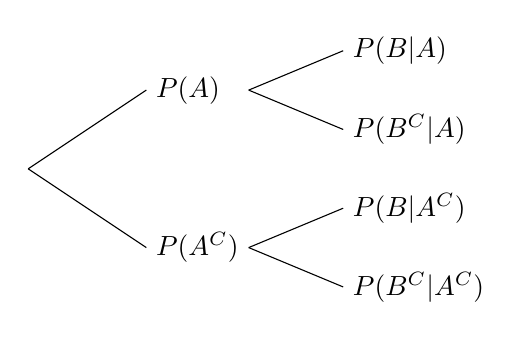
\begin{tikzpicture}
            \coordinate (O) at (0,0);
            \coordinate[label=right: $P(A)$] (AO) at (1.5,1);
            \coordinate[label=right: $P(A^C)$] (BO) at (1.5,-1);
            \coordinate (C1) at (2.8, 1);
            \coordinate (C2) at (2.8, -1);
            \coordinate[label=right: $P(B|A)$] (A1) at (4,1.5);
            \coordinate[label=right: $P(B^C|A)$] (B1) at (4,0.5);
            \coordinate[label=right: $P(B|A^C)$] (A2) at (4,-0.5);
            \coordinate[label=right: $P(B^C|A^C)$] (B2) at (4,-1.5);
            
            \draw (O) -- (AO);
            \draw (O) -- (BO);
            \draw (C1) -- (A1);
            \draw (C1) -- (B1);
            \draw (C2) -- (A2);
            \draw (C2) -- (B2);
        \end{tikzpicture}
    \end{subfigure}
\end{figure}

\end{document}


